\section{Einführung in das Thema}
Dieses Kapitel soll eine Einführung zum Thema SAT und 
FPGAs geben. In dem folgenden Unterkapitel
\ref{sec:intro_sat} wird auf das SAT-Problem, die 
zugrunde liegende Aussagenlogik und auf das in dieser
Arbeit benötigte Gruppieren von Formeln eingegangen.
Im Unterkapitel \ref{sec:sat_algo} wird der DPLL
Algorithmus als möglicher Lösungsansatz zum Lösen des SAT-Problems erläutert.
Grundlagen zum Thema FPGA werden im Unterkapitel 
\ref{sec:intro_fpga} vermittelt.

%%% EINFÜHRUNG SAT SOLVING %%%%%%%%%%%%%%%%%%%%%%%%%%%%
\subsection{Einführung in SAT}
\label{sec:intro_sat}
Im SAT-Problem oder auch Erfüllbarkeitsproblem
der Aussagenlogik wird die Frage gestellt ob eine
gegebene aussagenlogische Formel erfüllbar ist.
Das SAT-Problem is NP-vollständig, 
womit sich jedes Problem aus NP in
polynomieller Zeit auf SAT zurückführen lässt
\cite{cook:1971}. Somit gehört SAT auch zur Klasse NP
der Probleme, die in polynomieller Zeit mit einer
nichtdeterministischen Turingmaschine gelöst werden
können. Das Erfüllbarkeitsproblem ist nicht nur
komplexitätstheoretisch interessant, sondern auch
industrielle und wissenschaftliche Probleme können als
SAT-Problem formuliert werden. Um diese Probleme zu
lösen, wurden in den letzten Jahrzehnten effiziente 
Lösungsansätze entwickelt.\\
Bewährte Algorithmen zur Lösung von SAT sind DPLL, CDCL und SLS.
\begin{itemize}
\item
  \textbf{DPLL} \cite{davis:1962}\\
  Der Davis-Putnam-Logemann-Loveland (DPLL) Algorithmus
  ist Basis für eine Vielzahl von anderen
  SAT-Algorithmen und wird in dieser Arbeit verwendet.
\item
  \textbf{CDCL} \cite{mitchell:2004}\\
  Der Conflict Driven Clause Learning (CDCL) Algorithmus
  löst strukturierte Probleme besonders gut. Er baut
  auf DPLL auf und ist mithilfe vieler Verbesserungen
  heutiger Stand der Technik.
  
\item
  \textbf{SLS} \cite{hoos:2004}\\
  Mit Stochastik Local Search (SLS) Solvern kann nur
  die Erfüllbarkeit von Formeln gezeigt werden.
  Besonders zufällige Instanzen können mit dieser
  Art von Solvern effizient gelöst werden.
\end{itemize}


\subsubsection{Syntax der Aussagenlogik}
Das Alphabet $\Sigma$ der Aussagenlogik besteht aus 
einer (abzählbar) unendlichen Menge von 
aussagenlogischen Variablen ${\cal R} = \{p_1,p_1,\ ...\}$, 
einer Menge von Junktoren 
$\{\neg /1,\ \wedge /2,\ \vee /2,\ \rightarrow /2,\ \leftrightarrow /2\}$
und der Menge von Sonderzeichen $\{(,\ )\}$. Im Kontext
von SAT werden nur Formeln in konjunktiver Normalform
(KNF) betrachtet. Somit werden nur Begriffe in diesem 
Zusammenhang definiert. Da diese Definitionen Grundlagen
sind, wurden sie teilweise aus \cite{hoell:2009} übernommen.

  \begin{definition}
    Ein Atom ist eine aussagenlogische Variable.
   \end{definition}
  \begin{definition}
    Ein Literal ist eine aussagenlogische Variable oder
    eine negierte aussagenlogische Variable. Dabei wird
    eine aussagenlogische Variable auch positives Literal
    und eine negierte aussagenlogische Variable auch
    negatives Literal genannt.
  \end{definition}
  Im weiteren Verlauf werden
  Literale mit $l$ bezeichnet. Für konkrete Beispiele
  werden statt Buchstaben ganze Zahlen verwendet. Eine
  positive ganze Zahl entspricht einem positiven Literal,
  die gleiche ganze Zahl mit $-1$ multipliziert seiner
  Negation. Die Zahl 0 ist kein Literal, da sie weder
  negativ noch positiv ist. Ein Beispiel: 
  \begin{center}
    $l = 5$\\
    $\neg l = -5$
  \end{center}


  \begin{definition}
    Eine Klausel ist eine Disjunktion von Literalen.
  \end{definition}

  \begin{definition}
    Man nennt eine Klausel Unit oder Unit-Klausel, wenn
    sie nur aus einem Literal besteht. Dieses Literal wird 
    dann Unit-Literal genannt.
  \end{definition}
  \begin{definition}
    Eine Formel in KNF ist eine Konjunktion von Klauseln.
  \end{definition}
  \begin{function}
    Die Funktion $var(l)$, eines Literals $l$, gibt die
    ensprechende Variable von $l$ zurück.

  \end{function}
  \begin{function}
    Die Funktion $var(C)$ gibt die Menge von allen Variablen
    einer Klausel $C$ zurück.
  \end{function}
  \begin{function}
    Die Funktion $var(F)$ gibt die Menge von allen Variablen
    einer Formel $F$ zurück.
  \end{function}
  Klauseln werden ab jetzt immer mit dem Buchstaben $C$,
  Formeln mit $F$ und Literale mit $l$ dargestellt.
  Verschiedene Klauseln, Formeln bzw. Literale werden durch
  einen Index am Buchstaben unterschieden. Vereinfacht wird 
  eine Klausel statt 
  $((l_1 \vee l_2)\vee l_3)\vee ...\vee l_n)$
  in eckigen Klammern dargestellt 
  $[l_1, l_2, l_3,\ ..., l_n]$. Analog wird auch die 
  Schreibweise einer Formel in KNF vereinfacht. Statt 
  $((C_1 \wedge C_2)\wedge C_3)\wedge ...\wedge C_n)$ 
  schreibt man eine Formel wie folgt 
  $\langle C_1, C_2, C_3,\ ..., C_n \rangle$. Eine 
  Beispielformel könnte folgendermaßen aussehen.
  \begin{center}
    $F_{bsp} = \langle [1,3],[-2, 5, -6], [-1,-4,6], [-1,-2,-4,5], [-1,2]\rangle$
  \end{center}

  \subsubsection{Semantik der Aussagenlogik}
  Die Menge der Wahrheitswerte ${\cal W}$ ist die Menge
  $\{\top,\bot\}$. Dabei steht $\top$ für wahr und $\bot$
  für falsch. Man kann nun jeder aussagenlogischen Variable
  einen Wahrheitswert zuweisen. Verbindet man diese mit
  Junktoren zu Formeln, kann jeder Formel der Wert
  wahr oder falsch zuordnen werden, abhängig von den
  Wahrheitswerten der aussagenlogischen Variablen in der
  Formel.
  \begin{definition}
    Eine Interpretation ${\cal I}$ weist jeder
    aussagenlogischen Variable einer Formel einen
    Wahrheitswert zu.
    \begin{center}
    ${\cal I}: var(F)\rightarrow{\cal W}$
    \end{center}
  \end{definition}
  \begin{definition}
    Ein Literal ist erfüllt, wenn es eine
    aussagenlogische Variable ist, welche auf wahr
    abgebildet wird, oder eine negierte aussagenlogische
    Variable, welche auf falsch abgebildet wird.
  \end{definition}
  \begin{definition}
    Eine Klausel ist erfüllt, wenn mindestens ein Literal
    in der Klausel erfüllt ist. Die leere Klausel ist
    nach Definition unerfüllt.
  \end{definition}
  \begin{definition}
    Eine Formel ist erfüllt, wenn alle ihre Klauseln
    erfüllt sind. Eine leere Formel ist nach Definition
    immer erfüllt.
  \end{definition}
  \begin{definition}
    Eine partielle Interpretation ist eine
    Interpretation, welche nicht alle aussagenlogischen
    Variablen einer Formel $F$ auf einen Wahrheitswert
    abbildet.
  \end{definition}
  \begin{definition}
    Eine Interpretation, welche eine Formel $F$ erfüllt, 
    nennt man Modell von $F$.
  \end{definition}
  %% Eine partielle Interpretation kann auch als Menge von
  %% Literalen verstanden werden. Alle Literale in dieser Menge
  %% der partiellen Interpretation werden auf wahr und deren
  %% Negation auf falsch abgebildet. Undefiniert nennt man Variablen, wenn diese nicht
  %% in der partiellen Interpretation vorhanden sind.
  Eine partielle Interpretation wird als Liste von
  Literalen, welche auf wahr abgebildet werden,
  dargestellt. Sollte ein Literal oder seine Negation
  nicht in dieser Liste vorhanden sein, dann ist ihr Wahrheitswert
  undefiniert. Die Sortierung der partiellen
  Interpretation ist wichtig, da sie den aktuellen Pfad 
  im Suchbaum widerspiegelt. Ist zum Beispiel folgende
  partielle Interpretation gegeben $(l_1,l_2, ..., l_n)$,
  dann wurde das Literal $l_1$ im Suchprozess zuerst
  entschieden und  $l_n$ zuletzt. Eine partielle Interpretation,
  welche alle Variablen eine Formel enthält, nennt man total.\\
  \begin{definition}
    Ist $F$ eine Formel und $J$ eine partielle oder totale Interpretation, 
    dann ist $F|_J$ das Redukt bzw. das verbleibende
    Problem der Formel. 
  \end{definition}
  Das Redukt wird wie folgt gebildet:
    \begin{itemize}
      \item Alle Klauseln, welche mindestens ein erfülltes Literal
        aus $J$ enthalten, werden aus $F$ entfernt.
      \item Alle Literale, welche negiert in $J$ vorkommen,
        werden aus ihren Klauseln in $F$ entfernt.
    \end{itemize}
  Sei  nun die Formel $F_{bsp}$ aus dem
  vorherigen Abschnitt zusammen mit der partiellen
  Interpretation $J = (-1,-5)$ gegeben, dann ist
  $F_{bsp}|_J = \langle [3],[-2,-6]\rangle$
  das Redukt von $F_{bsp}$ unter $J$. Die Klausel 
  $[3] \in F_{bsp}|_J$ ist eine Unit-Klausel,
  mit dem Unit-Literal 3.


  \subsubsection{Gruppieren von Klauseln}
  Für das Lösen einer SAT-Instanz mit dem später
  vorgestellten Entwurf ist es nötig, die Formel in
  Gruppen von Klauseln zu unterteilen. Diese Gruppen
  haben die Eigenschaft, dass jede Variable maximal einmal
  vorkommt. Daraus folgt,
  das man maximal ein Literal pro Gruppe nach einem
  Inferenzprozess erhält. Es werden nun Begriffe
  definiert, die für die Gruppierung von Formeln 
  benötigt werden.
  \begin{definition}
    Eine Gruppe ist eine Menge von Klauseln.
    \begin{center}
      $G = \{C_1, ..., C_m\}$
    \end{center}
  \end{definition}

  \begin{function}
    Die Funktion $occ(v, G)$ berechnet die Anzahl der Vorkommen einer
    Variable $v$ in einer Gruppe $G$.
    \begin{center}
      $occ(v, G) = |\{C \mid C \in G, v \in var(C)\}|$
    \end{center}
  \end{function}

  \begin{definition}
    ${\cal G}^{(i)}$ ist eine Menge
    von Gruppen mit maximalem Variablen Vorkommen von $i$.
    \begin{center}
      ${\cal G}^{(i)} = \{G_1, ..., Gn\}$
    \end{center}
    Es gilt:
    \begin{itemize}
      \item
        ${\cal G}^{(i)}$ ist eine endliche Menge von 
        Gruppen $:\ |{\cal G}^{(i)}| \leq n$
      \item
        $\forall G \in {\cal G}^{(i)} : occ(v,G) \leq i$
    \end{itemize}
  \end{definition}

  \begin{function}
    Die Funktion $group: F \rightarrow {\cal G}^{(i)}$ ist
    eine bijektive Abbildung aus einer Menge von Klauseln (Formel) in die
    Menge von Gruppen. Es wird  jeder Klausel einer Formel 
    eindeutig eine Gruppe zugewiesen.

  \end{function}
  Die Anzahl von Vorkommen von Variablen in Gruppen wird
  im Weiteren auf $i = 1$ beschränkt. Damit ergeben sich
  die folgenden Eigenschaften.

  \begin{definition}
  Die Funktion $f: V \rightarrow {\cal N}_0$ ist die
  Knotenfärbung eines Graphen $G(V,E)$ ohne
  Mehrfachkanten. Man nennt $f$ gültig oder zulässig,
  falls zwei beliebige benachbarte Knoten nicht
  dieselbe Farbe besitzen. 
  \end{definition}
  Analog dazu ist auch 
  $group: {\cal C} \rightarrow {\cal G}^{(1)}$ eine
  Knotenfärbungsfunktion eines Graphen $G(F, Var)$,
  $Var = \{(C_x,C_y)\mid C_x, C_y \in F, \exists\ v \in var(F),\ v \in var(C_x), v \in var(C_y)\}$.
  Knoten des Graphen entprechen den Klausel von $F$,
  wobei zwei Knoten durch eine Kante verbunden 
  werden, wenn gleiche Variablen geteilt werden.
  Man nennt $group$ gültig oder zulässig,
  falls zwei beliebige benachbarte Knoten nicht
  dieselbe Gruppe besitzen. 
  Eine Formel $F_{group} = \langle C_1, C_2, C_3,C_4 \rangle =  \langle[1,2],[2,3],[3,4],[4,5]\rangle$
  entspricht dem Graphen in Abbildung \ref{formula}
  und kann mit $group: {\cal C} \rightarrow {\cal G}^{(1)}$
  auf verschiedene Weise in zwei verschiedene Farben
  (Gruppen) gefärbt werden (Abbildung \ref{formula_colored}).
  \begin{figure}[h]
    \centering
    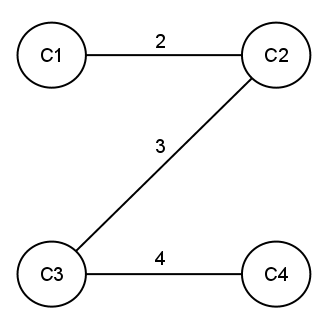
\includegraphics[width=0.25\textwidth]{abb/formula_graph.png}
    \caption{Graph zur Formel $F_{group}$}
    \label{formula}
  \end{figure}
   \begin{figure}[h]
    \centering
    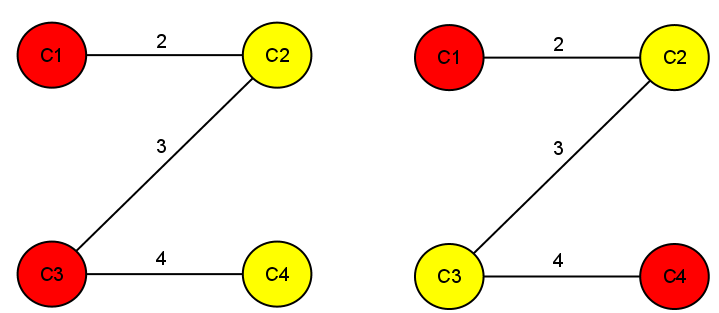
\includegraphics[width=0.5\textwidth]{abb/formula_graph_colored.png}
    \caption{Mögliche Färbung des Graphen zur Formel $F_{group}$}
    \label{formula_colored}
  \end{figure}
  Wenn ein Graph färbbar ist, gibt es eine kleinste
  Zahl $k$, sodass der Graph $k$-knoten-färbbar ist. 
  Diese Zahl wird die chromatische Zahl oder
  Knotenfärbungszahl des Graphen genannt und meist mit 
  $\chi(G)$ bezeichnet. Existiert für endlich viele
  Farben keine Färbung setzt man symbolisch $\chi(G)=\infty$.
  Die Bestimmung der chromatischen Zahl eines Graphen ist
  NP-schwer, das heißt, dass es aus Sicht der Komplexitätstheorie 
  vermutlich keinen Algorithmus gibt, der dieses Problem 
  effizient löst. Das bedeutet auch, dass die Bestimmung der
  kleinsten Anzahl n von Gruppen in ${\cal G}^{(1)}$ ein
  NP-schweres Problem ist.\\
  Für größere SAT Probleme, ist eine 
  intelligente Heuristiken nötig um ein schnelles Gruppieren
  zu gewährleisten.

%%% Algorithmen zum lösen des SAT Problems %%%%%%%%%%%%
\subsection{Lösen des SAT-Problems}
\label{sec:sat_algo}
Dieses Unterkapitel beschreibt den bereits seit 1962
existierenden DPLL-Algorithmus \cite{davis:1960}.
Ursprünglich wurde dieser 
Algorithmus eingesetzt, um Unerfüllbarkeit zu zeigen. 
In dieser Arbeit wird eine Version vorgestellt, welche die
Lösbarkeit von Formeln zeigt.\\
%\todo{bessere Einleitung}\\

\subsubsection{Suchbäume}
Ein Suchbaum ist ein binärer Baum. Jeder Knoten $t$ hat
genau zwei Nachfolgeknoten $t_1$ und $t_2$. Kanten zwischen zwei Knoten werden
mit Literalen beschriftet. Ist eine Kante $t \rightarrow t_1$ zu einem
Kindsknoten mit $l$ beschriftet, dann muss die Kante $t \rightarrow t_2$
zu dem anderen Kindsknoten mit $\neg l$ beschriftet sein. Desweiteren
darf die Variable des Literals, welche zur Beschriftung einer Kante benutzt
wurde, nicht bereits auf dem Pfad vom Wurzelknoten zum Knoten $t$ benutzt
worden sein.
 \begin{figure}[h]
    \centering
    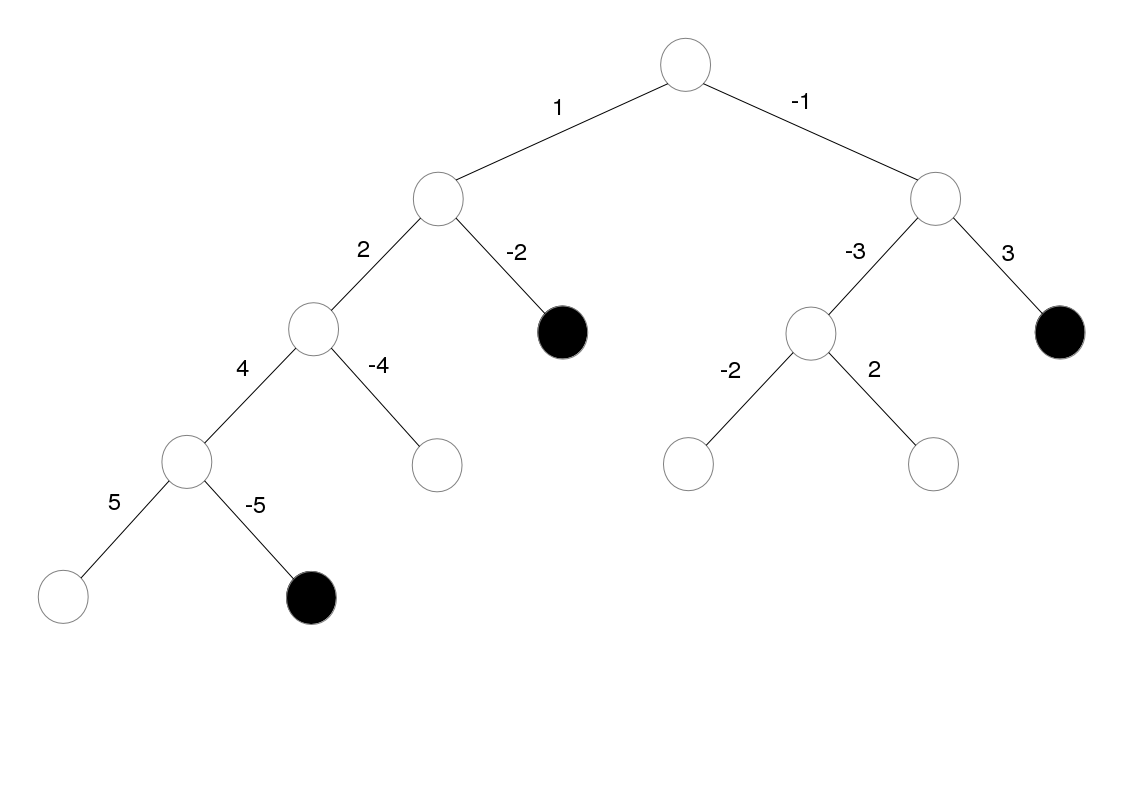
\includegraphics[width=\textwidth]{abb/suchbaum.png}
    \caption{Beispiel für einen Suchbaum}
    \label{suchbaum}
  \end{figure}
Der Pfad von einem Knoten $t$ zum Wurzelknoten entspricht der partiellen
Interpretation, welche alle Literale auf diesem Pfad enthält. Die Suche
kann auf einem Pfad beendet werden, wenn die partielle Interpretation 
des Pfades jedes Literal einer Klausel $C$ der Formel $F$ nicht erfüllt. Da bereits alle
Literale, welche $C$ enthält, auf dem Pfad vorkommen und $C$ weder
undefiniert noch erfüllte Literale enthält, kann man $F$ nicht erfüllen,
indem man weitere Literale zum aktuellen Suchpfad hinzufügt. Deshalb
kann dieser Pfad geschlossen werden. Sollte ein Pfad alle
Variablen von $F$ enthalten und alle Klauseln erfüllen,
dann ist die entsprechende Interpretation ein Modell
von $F$.\\
Ein Suchbaum wird also solange durch Hinzufügen
von neuen Kindsknoten erweitert, bis ein Pfad gefunden wurde, welcher
alle Variablen enthält, oder alle Pfade mit einer
unerfüllten Klausel enden. Wurde ein Modell gefunden, dann ist
die Formel erfüllbar.\\
Abbildung \ref{suchbaum} zeigt einen nicht vollständig expandierten
Suchbaum der Beispielformel $F_{bsp}$. Schwarze Knoten im Baum 
stellen nicht erfüllende Pfade dar.

\subsubsection{Davis Putnam Logemann Loveland Algorithmus}
Der Davis Putnam Logemann Loveland (DPLL) Algorithmus
erzeugt mithilfe von speziellen Regeln einen Suchbaum.
In Abbildung \ref{dpll} ist der Algorithmus als Flussdiagramm
angegeben. 
 \begin{figure}[h!]
    \centering
    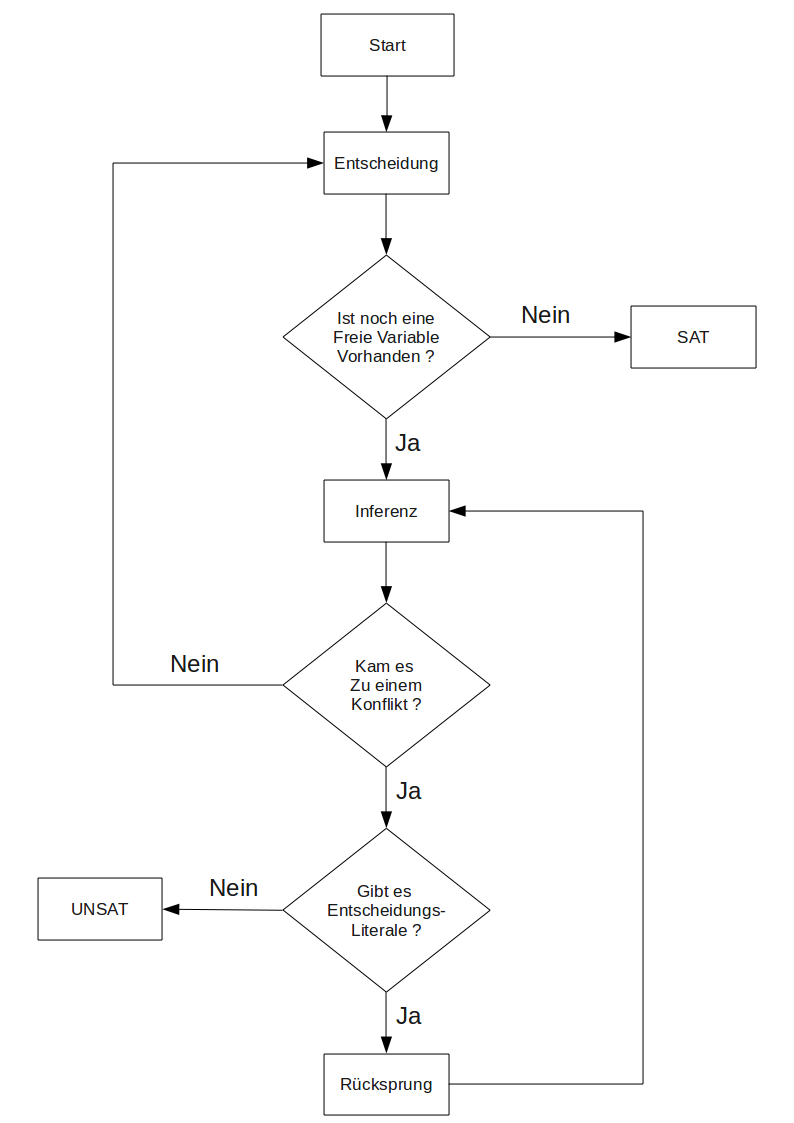
\includegraphics[width=0.75\textwidth]{abb/dpll.png}
    \caption{Flussdiagramm des DPLL-Algorithmus}
    \label{dpll}
  \end{figure}
Unit Literale in der Ausgangsformel
können der partiellen Interpretation hinzugefügt werden.
Es wird damit begonnen, sich für eine freie Variable
zu entscheiden, das heißt eine Variable oder die negierte
Variable, welche noch nicht in der partiellen Interpretation
enthalten ist, wird auf wahr abgebildet. Das Literal wird 
Entscheidungsliteral genannt. Sollte keine freie
Variable mehr vorhanden sein, dann beendet man den Prozess
mit SAT. Wenn sich für eine Variable entschieden wurde, dann 
wird mit der Inferenz der Formel begonnen. Im Inferenzprozess 
sucht man nach Unit-Klauseln im Redukt der Formel. Findet
man unter der aktuellen partiellen Interpretation
eine solche Unit, wird das Literal dieser Klausel
der partiellen Interpretation hinzugefügt und der Inferenzprozess
beginnt erneut. Dies geht solange, bis das Redukt der 
Formel keine Units mehr enthält. Kommt es nicht zum
Konflikt entscheidet man sich für die nächste Variable.
Sollte das Redukt jedoch eine leere Klausel enthalten, 
bedeutet dies, dass alle Literale der Klausel nicht
erfüllt sind und somit die Klausel bzw. die Formel nicht 
erfüllt ist (Konflikt). Wenn sich kein Entscheidungsliteral
in der partiellen Interpretation befindet, dann wird
der Prozess mit ``nicht erfüllbar'' (UNSAT) beendet. Ist mindestens ein
Entscheidungsliteral vorhanden, dann werden alle
Literale bis zu diesem Literal von der partiellen 
Interpretation entfernt und das negierte Entscheidungsliteral
wieder hinzugefügt. Dieses negierte Literal ist selbst
kein Entscheidungsliteral mehr. Nach dem sogenannten Rücksprung
wird wieder eine Inferenz 
der Formel angestoßen.
 \begin{figure}[h!]
    \centering
    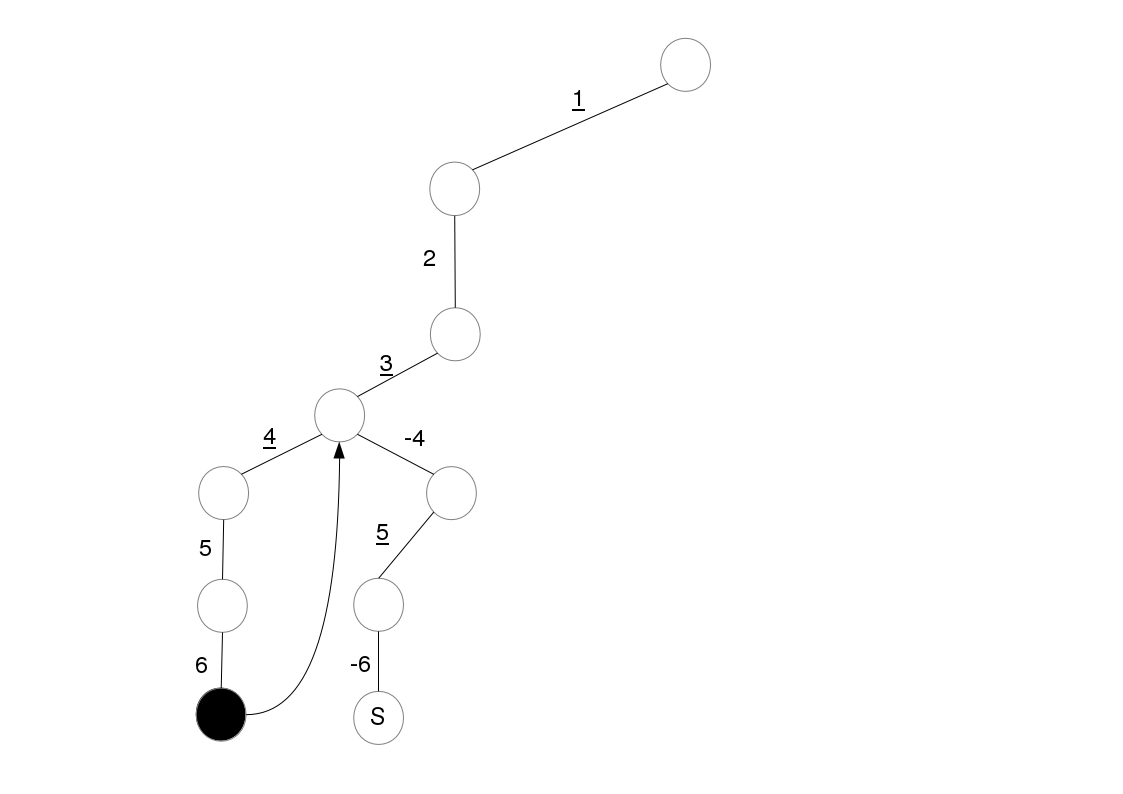
\includegraphics[width=\textwidth]{abb/dpll-suchbaum.png}
    \caption{DPLL-Suchbaum}
    \label{dpll-suchbaum}
  \end{figure}
Wendet man nun den vorgestellten DPLL-Algorithmus aus Abbildung
\ref{dpll} auf $F_{bsp}$ an, entsteht der Suchbaum in Abbildung
\ref{dpll-suchbaum}. Die Entscheidungsheuristik entscheidet 
sich in diesem Beispiel immer für die kleinste freie Variable.
Dieser Suchbaum weißt die Besonderheit auf,
dass manche Knoten nur einen Kindsknoten besitzen. Dies folgt
aus der Inferenz der Formel, da man gezwungen ist
Literalen einen gewissen Wahrheitswert zuzuweisen, um die Klausel zu
erfüllen. Literale welche im Suchbaum unterstrichen sind, 
sind Entscheidungsliterale. Werden Pfade mit S beschriftet, 
dann ist die partielle Interpretation dieses Pfades ein 
Modell der Formel.


\subsection{Einführung in FPGAs}
\label{sec:intro_fpga}
Ein Field Programmable Gate Array (FPGA) besteht 
hauptsächlich aus Speichern (FlipFlops \cite{scarbata:2001}) 
und davor geschaltenen Logikelementen,
welche in einer Matrix angeordnet sind.
Diese Logikelmente sind LUTs
(Lookup Tables), die über eine Programmierung die
gewünschte Funktion realisieren. Abbildung \ref{fpga} 
skizziert den Aufbau eines FPGA-Schaltkreises.
\begin{figure}[h]
  \centering
  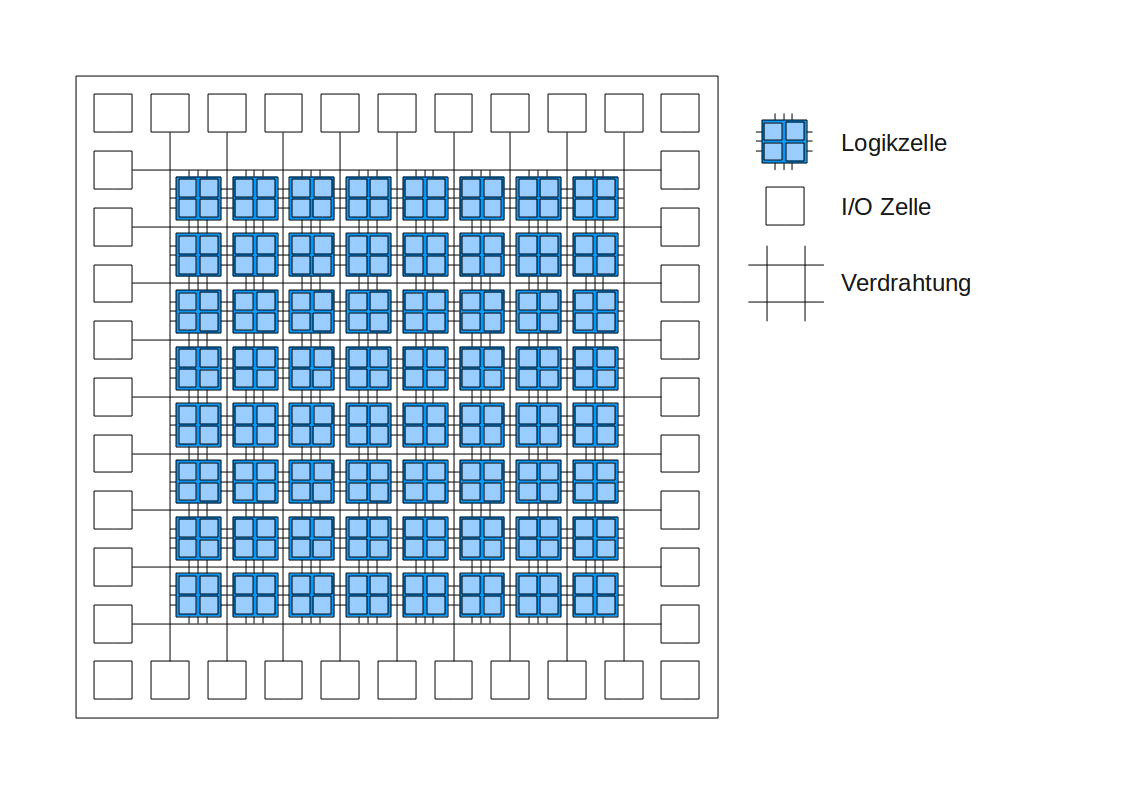
\includegraphics[width=\textwidth]{abb/fpga.png}
  \caption{FPGA-Skizze}
  \label{fpga}
\end{figure}
Eine LUT mit k Eingängen kann eine beliebige k-stellige
Binärfunktion realisieren. Die Anzahl von
Eingangssignalen pro LUT ist vom FPGA abhängig
und liegt meist zwischen 4 und 6 Eingangssignalen.
LUTs mit mehr Eingängen werden in der Regel nicht
gefertigt, da diese eine potenziell schlechtere
Auslastung aufweisen. Für Funktionen, die mehr
Eingänge erfordern als eine einzige LUT bietet,
werden mehrere LUTs direkt miteinander verschaltet.
Die Programmierung der gewünschten Funktion erfolgt
durch die Hinterlegung der definierenden Wahrheitstabelle
in den Speicher-Zellen der LUT, die Funktionsberechnung 
durch das Auslesen der durch die Eingänge bestimmten
Speicheradresse. Die Speicher sind in den meisten
FPGAs durch SRAM-Speicherzellen realisiert, welche
beim Konfigurationsprozess geladen werden.
Das Laden dieser Konfigurationsdaten bzw.
Verknüpfungsregeln geschieht dabei in der Regel aus
einem speziellen Flash-ROM Baustein heraus. Man kann den
FPGA über entsprechende Schnittstellen (JTAG \cite{ieeejtag:1990}),
konfigurieren um dessen Funktion zu implementieren.
Im Allgemeinen sind LUTs nur lesbar, es gibt jedoch auch Erweiterungen,
mit denen die Speicher der LUTs ebenfalls beschrieben
werden können.
Diese Technologie heißt Distributed RAM.
Abbildung \ref{lut} zeigt eine LUT mit
4 Eingängen und ein dahinter geschaltener FlipFlop.
\begin{figure}[h]
  \centering
  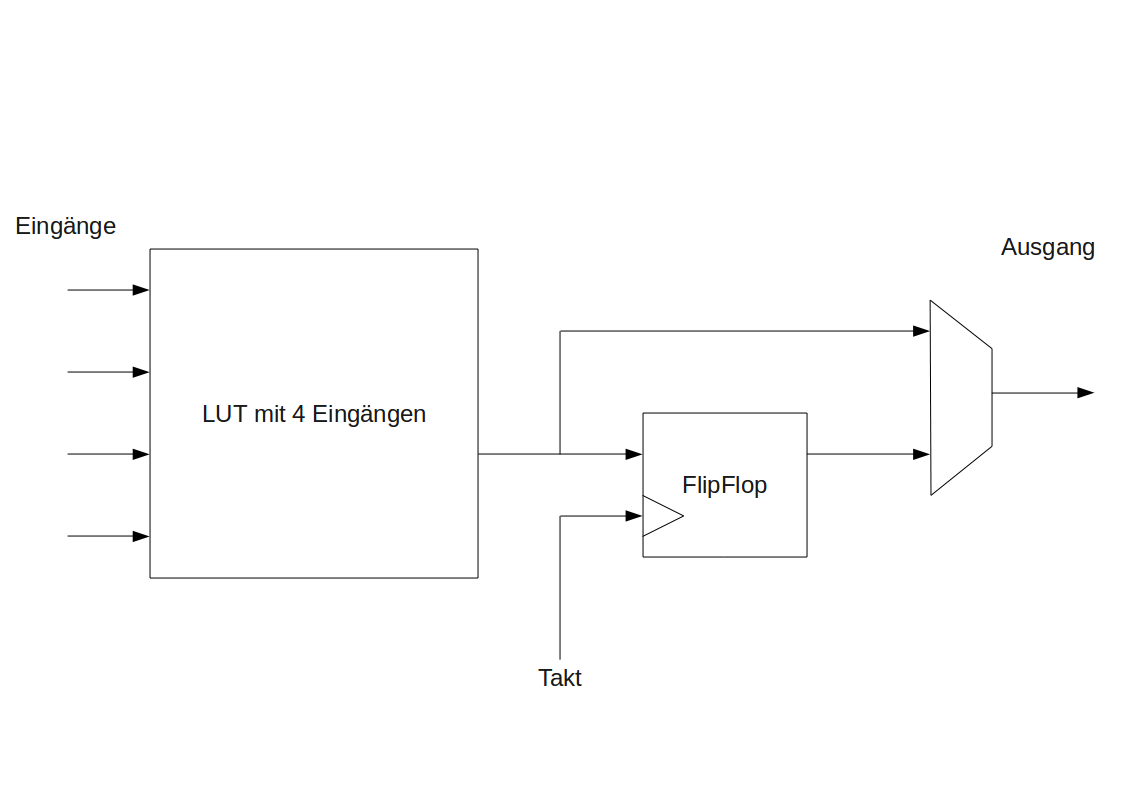
\includegraphics[width=\textwidth]{abb/logikzelle.png}
  \caption{Einfache Logikzelle}
  \label{lut}
\end{figure}
Die FlipFlops dienen dazu, Signalwerte
zwischenzuspeichern, um sie im nächsten Takt
weiterverarbeiten zu können. Meist wird
jeder LUT genau ein FlipFlop zugeordnet.
Eine Kombination von FlipFlop und Logikelement
wird zu einer Logikzelle (CLB) zusammengefasst.
Es können auch mehrere LUTs / FlipFlops in einer
Logikzelle zusammengefasst werden, dies variiert von
Hersteller zu Hersteller. Aktuelle FPGAs bestehen aus
mehreren zehntausend Logikzellen. Alle LUTs arbeiten
unabhängig voneinander und somit parallel.\\
Neben den Logikzellen beinhalten FPGAs darüberhinaus
komplexe Verdrahtungsnetzwerke, um Logikzellen auf
gewünschte Weise zu verbinden. Desweiteren stehen
meist noch zusätzliche Funktionsblöcke 
(auch Hard Macros genannt) zur Verfügung, welche bereits
eine vordefinierte Funktion erfüllen. Dies sind zum Beispiel
Multiplizierer, Taktgeneratoren \\ oder Block-RAMs \cite{xilinxbram:2005}.\\
Block-RAMs sind verteilte Speicher auf dem FPGA und lassen sich
auf vielfältige Weise ansprechen. So können 
damit Single- oder Dualport-RAMs mit variabler Bitbreite
erzeugt werden. Üblich sind mehrere kleinere 
Dualport-Block-RAMs von 18Kbit (Xilinx FPGAs).\\ 
Der FPGA-Chip wird von
einer Vielzahl von I/O Blöcken umrandet. I/O Zellen dienen der
Kommunikation mit der Außenwelt. Über I/O Blöcke werden
die Anschlüsse des FPGAs mit der Schaltmatrix verbunden.
Auch diese I/O Blöcke können an die jeweilige Anwendung
angepasst werden, z. B. kann die Ausgangsspannung an
den jeweiligen Standard angepasst \\werden (TTL/CMOS usw.).\\
Programmiert bzw. konfiguriert wird der FPGA mittels
einer Hardwarebeschreibungssprache (HDL) wie VHDL oder Verilog. 
Die Speicherbelegung der Logikzellen übernimmt dabei ein
Synthesewerkzeug, welches aus dem HDL-Quelltext die
Konfiguration synthetisiert.


